\documentclass[a4paper]{article}
\usepackage[utf8]{inputenc}
\usepackage[spanish]{babel}
\usepackage{amssymb,amsmath,amsbsy}
\usepackage{url}
\usepackage[parfill]{parskip}
\usepackage[pdftex]{graphicx}
\usepackage{subfigure}
\usepackage{float}
\usepackage{subfig}
\usepackage{listings}
\usepackage{multirow}
\usepackage{vmargin}
\usepackage{tcolorbox}
\usepackage{mathabx}
\usepackage{slashbox}
\usepackage{fancyhdr}
\usepackage{enumerate}
\usepackage{lastpage}
\usepackage{amsmath,lipsum}


\newcommand{\HRule}{\rule{\linewidth}{0.5mm}}
\DeclareGraphicsExtensions{.jpg}
\DeclareGraphicsExtensions{.png}
\numberwithin{equation}{section}
\numberwithin{figure}{section}
\setcounter{secnumdepth}{4}
\setlength{\parindent}{1cm}
\setmargins{2.5cm}       
{0.5cm}                        
{16.5cm}                      
{23.92cm}                
{10pt}                         
{1cm}                         
{0pt}                            
{1.5cm} 
   
\begin{document}
%CARATULA
\begin{titlepage}
\begin{center}
\begin{figure}[H]\label{cranio}
\centering

\includegraphics[width=0.5\textwidth]{cranio}
\end{figure}
\begin{minipage}[t]{0.5\textwidth}
\begin{flushright} 


  \huge
\LARGE  \ \\[3.8cm]
\noindent

\noindent
\end{flushright}
\end{minipage}
\HRule \\[1cm]
\noindent
\textsc{\LARGE Hogareña}\\[1.5cm]
\textsc{\Large  Información técnica}\\[0.7cm]
\HRule \\[1cm]
\noindent

\vfill
\end{center}
\end{titlepage}
%FIN CARATULA

\tableofcontents

\pagebreak
\section{Componentes}
\begin{itemize}

\item Cable plano 14 hilos (Longuitud segun disposición de las placas)
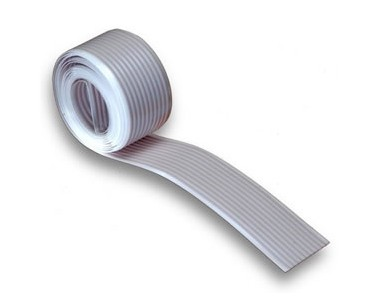
\includegraphics[width=0.07\textwidth]{cable_plano.png}
\item Hembra cable plano para 14 hilos (x 2 Unidades)
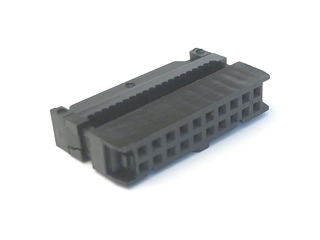
\includegraphics[width=0.07\textwidth]{hembra_cable_plano.png}
\item Pulsador Normalmente Abierto (x2 Unidades, Set de temperatura)

\item Cable de 2 hilos (Longitud necesaria segun disposición de los pulsadores)
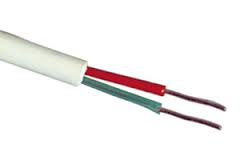
\includegraphics[width=0.07\textwidth]{cable_2_hilos.png}
\item Hembra de 2 vias para pines (x2 Unidades, Pulsador)
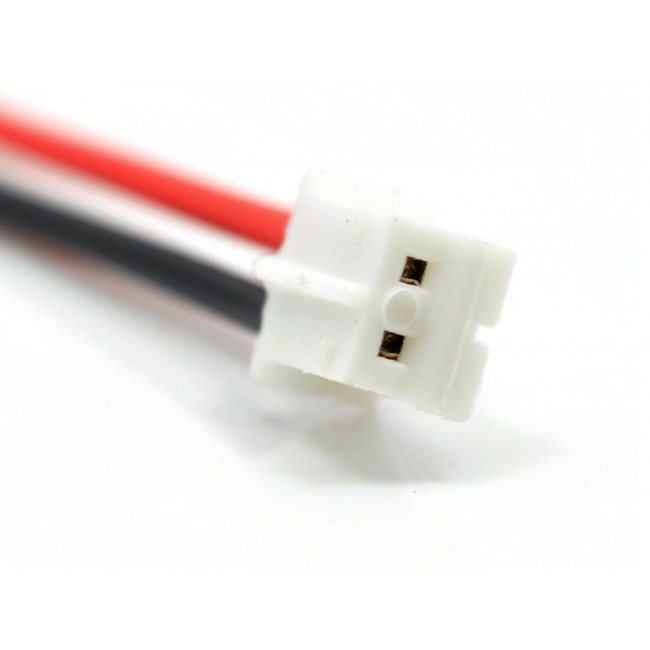
\includegraphics[width=0.07\textwidth]{hembra_2.png}
\item Hembra Housing x2 Vias (x1 Unidad, Alimentación)
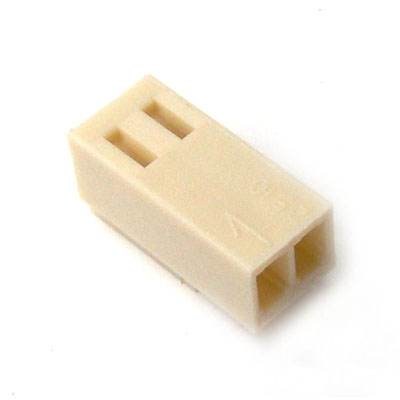
\includegraphics[width=0.07\textwidth]{hembra_housing.png}
\item Hembra Housing x3 Vias (x2 Unidades, Sensor de temperatura,$I^{2}C$)
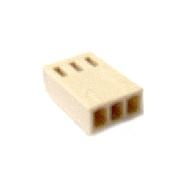
\includegraphics[width=0.07\textwidth]{hembra_housing_3.png} 
\item Cooler 14V AGREGAR MEDIDAS(x2 Unidades)
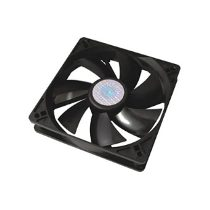
\includegraphics[width=0.07\textwidth]{cooler.png}
\item Cable conexiones cooler, celda peltier (Longitud segun disposición)
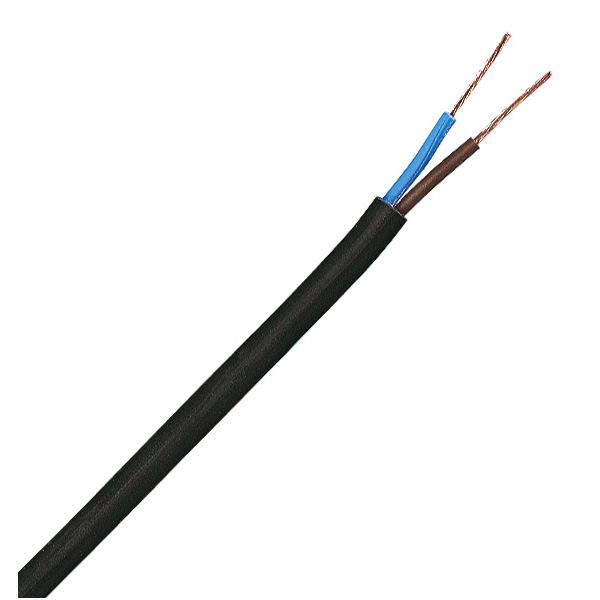
\includegraphics[width=0.07\textwidth]{cable_2mm.png}
\item Celda Peltier (x4 Unidades)
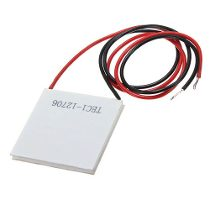
\includegraphics[width=0.07\textwidth]{celda_peltier.png}
\item Motor de Continua 12V 0,6A Corriente Nominal (x2 Unidades)
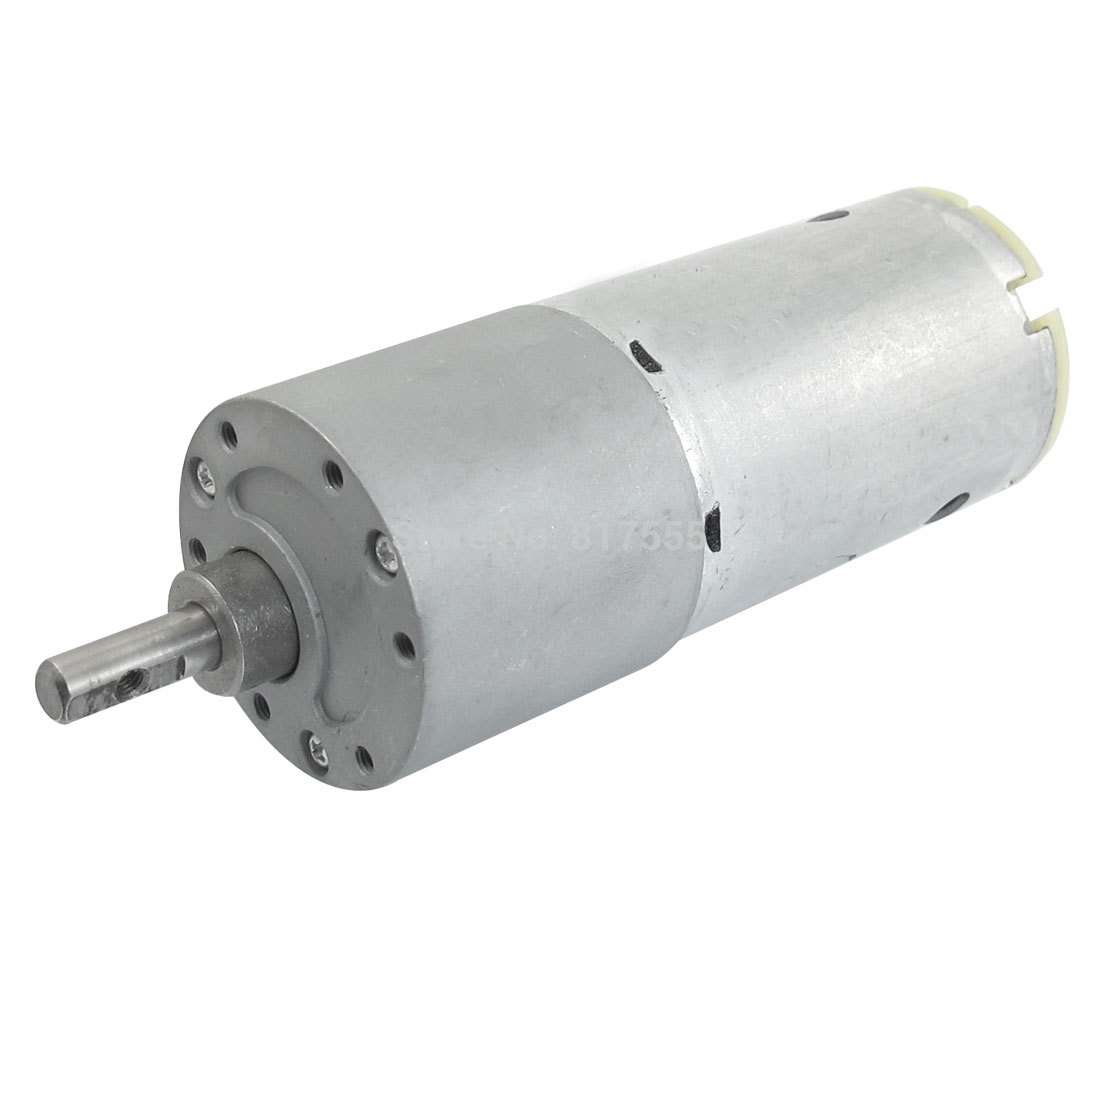
\includegraphics[width=0.07\textwidth]{motor.png}	


\subsection{Disipadores}
\begin{itemize}
\item Disipador interno Celda Peltier (x1 Unidad) 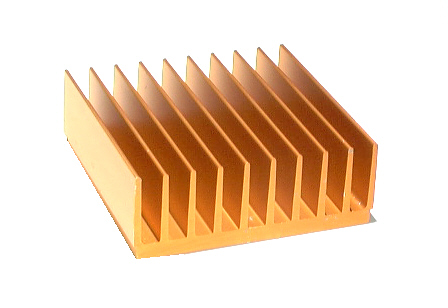
\includegraphics[width=0.07\textwidth]{disipador_externo.png}	
\item Disipador externo Celda Peltier (x1 Unidad)
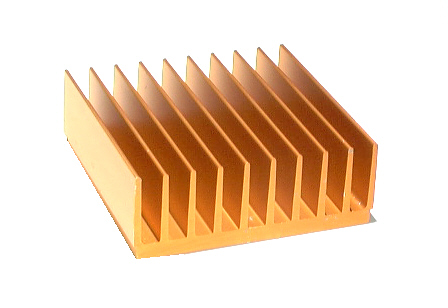
\includegraphics[width=0.07\textwidth]{disipador_externo.png}	
\item Disipador LM7805 (x 1 Unidad, 15x15x15)
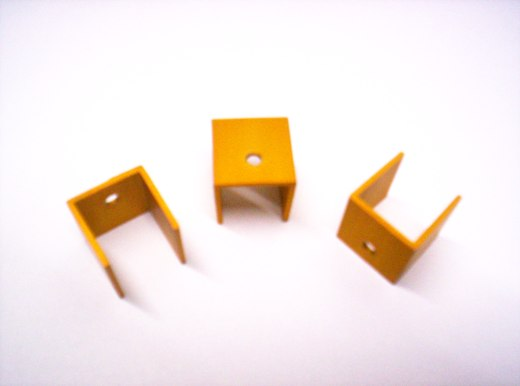
\includegraphics[width=0.07\textwidth]{disipar_lm.png}	
\end{itemize}

\subsection {HTC Display Board}
\begin{itemize}
\item Placa HTC Display Board (x1 Unidad)
\item 7 Segment (x2 Unidades, THT-DIP16-Catodo Común)
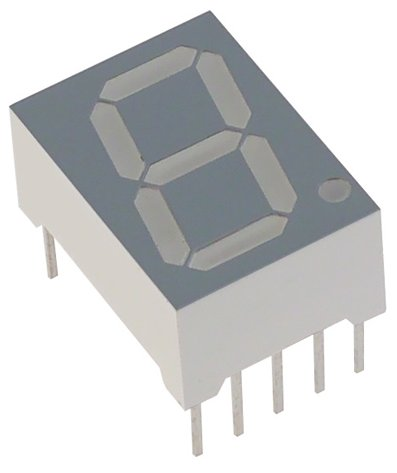
\includegraphics[width=0.07\textwidth]{7segment.png}	
\item 74LS48 (x2 Unidades, THT- BCDto7SEG)
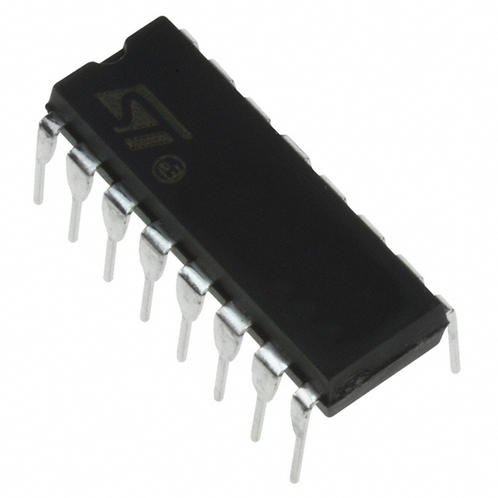
\includegraphics[width=0.07\textwidth]{74ls48.png}	


\subsubsection {Headers}
\begin{itemize}
\item Tira de pines doble (x1 Unidad)
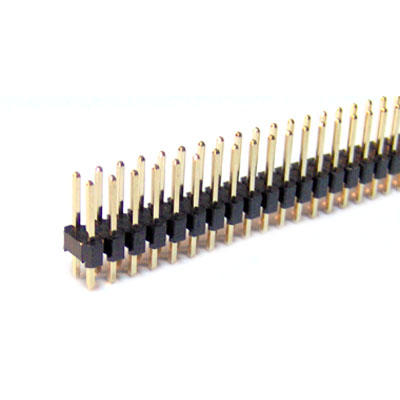
\includegraphics[width=0.07\textwidth]{tira_de_pines.png}	
\end{itemize}

\subsubsection {Capacitores SMD-0805}
\begin{itemize}
\item $100nF$ (x2 Unidades)
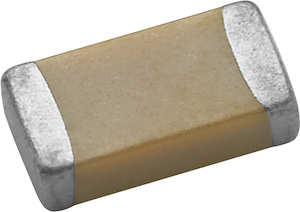
\includegraphics[width=0.03\textwidth]{capacitor_smd.png}	
\item $1nF$ (x2 Unidades)
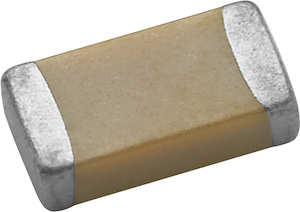
\includegraphics[width=0.03\textwidth]{capacitor_smd.png}	
\end{itemize}

\subsubsection {Resistencias SMD-0805}
\begin{itemize}
\item $330\Omega$ (x14 Unidades)
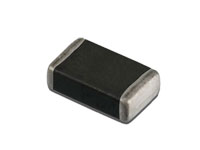
\includegraphics[width=0.03\textwidth]{resistencia_smd.png}	
\end{itemize}
\end{itemize}
\subsection {HTC Control Board}
\begin{itemize}


\item Placa HTC Control Board (x1 Unidad)

\item Bornera 2 vias (x3 Unidades)
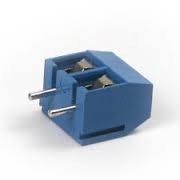
\includegraphics[width=0.07\textwidth]{bornera.png}	
\item CNY74-2 (x1 Unidad, THT-Optoacoplador)
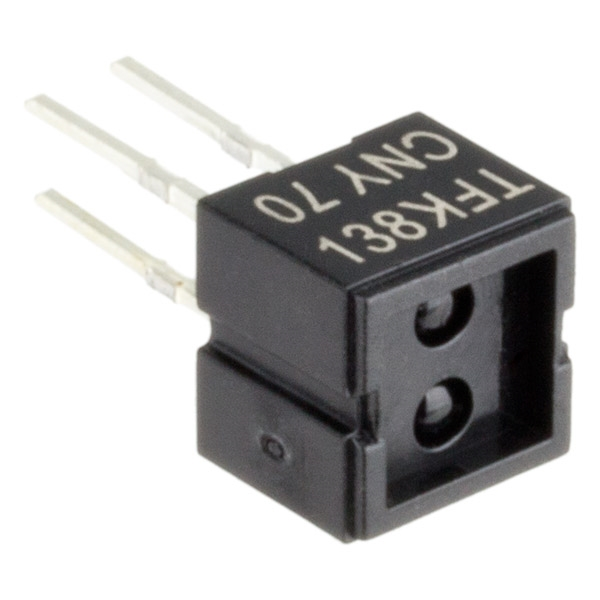
\includegraphics[width=0.07\textwidth]{cny70.png}	
\item LED Verde (x1 Unidad, SMD-0805)
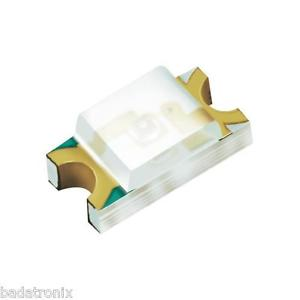
\includegraphics[width=0.07\textwidth]{led_verde.png}	
\item Diodo 1N4148 (x2 Unidades, SMD-1206)
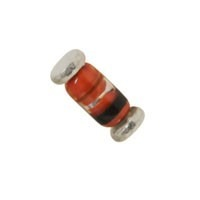
\includegraphics[width=0.07\textwidth]{diodo_smd.png}	
\item LM7805 (x1 Unidad, THT)
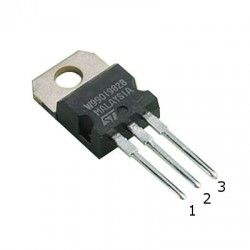
\includegraphics[width=0.07\textwidth]{lm7805.png}	
\item MSP430G2553 (x1 Unidad)
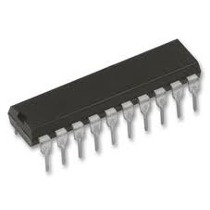
\includegraphics[width=0.07\textwidth]{msp.png}	
\item Zocalo para 20 pines (x1 Unidad)
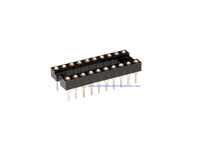
\includegraphics[width=0.07\textwidth]{zocalo.png}	
\item DS18B20 (x1 Unidad)
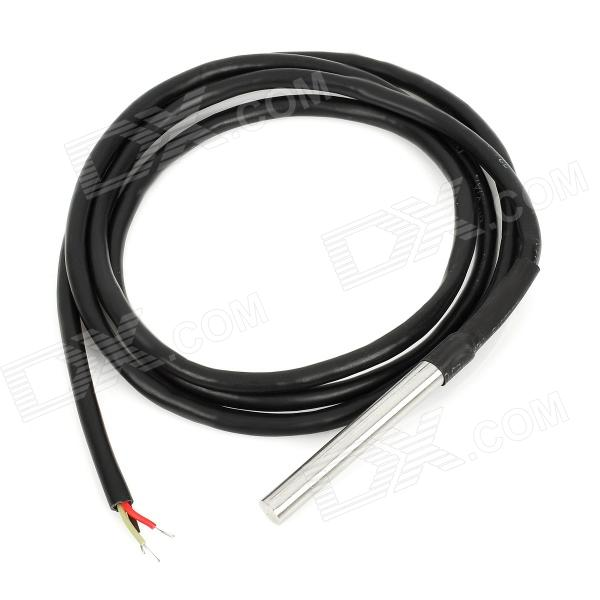
\includegraphics[width=0.1\textwidth]{ds18b20.png}	
\item AIC/LM1117 (x1 Unidad, SOT-223)
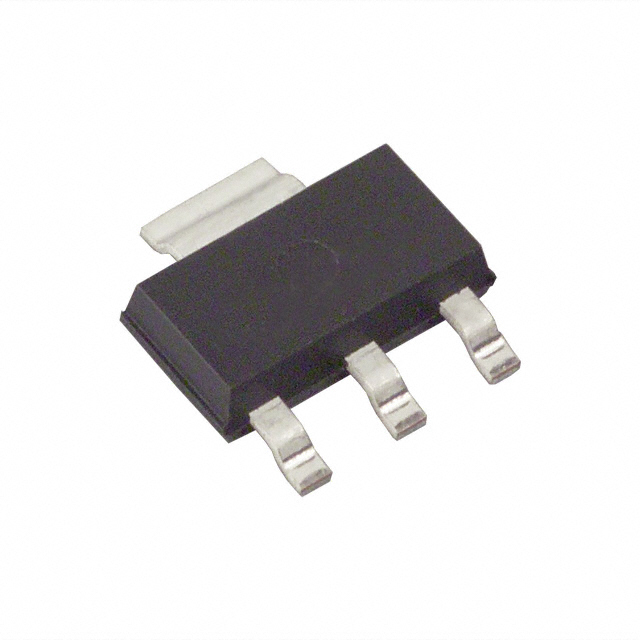
\includegraphics[width=0.07\textwidth]{sot223.png}	
\item Relay SRD-05VDC-SL-C (x2 Unidades)
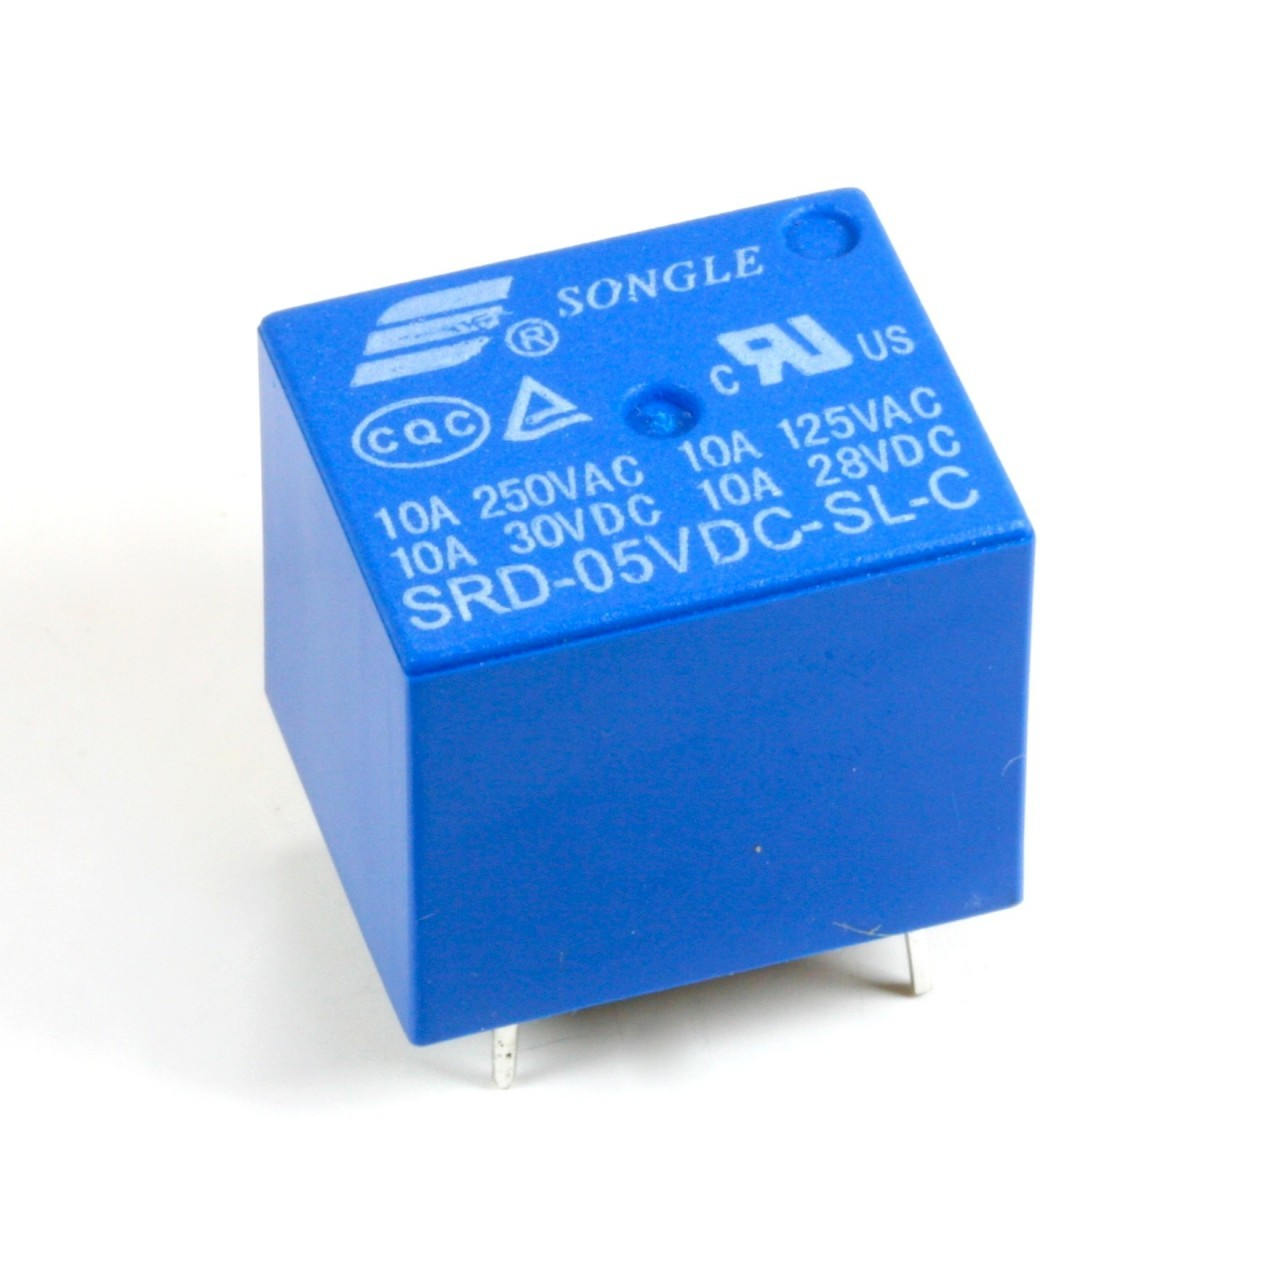
\includegraphics[width=0.07\textwidth]{relay.png}	
\item 2N3904 (x2 Unidades, NPN Transistor, TO92)
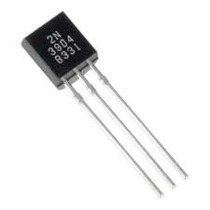
\includegraphics[width=0.07\textwidth]{2n3904.png}	1
\end{itemize}

\subsubsection {Headers}
\begin{itemize}
\item Macho Housing x2 vias (x1 Unidad, Alimentación)
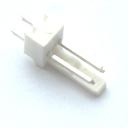
\includegraphics[width=0.07\textwidth]{housing_2.png}	
\item Macho Housing x3 vias (x2 Unidades, Sensor de temperatura, $I^{2}C$)
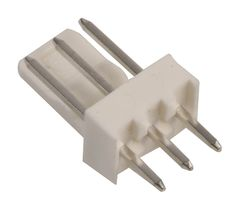
\includegraphics[width=0.07\textwidth]{housing_3.png}	
\item Tira de pines doble (x1 Unidad)
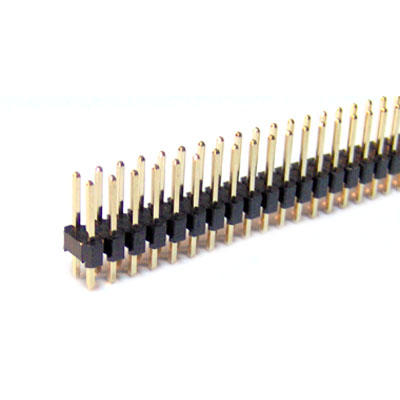
\includegraphics[width=0.07\textwidth]{tira_de_pines.png}	
\item Tira de pines simple (x1 Unidad)
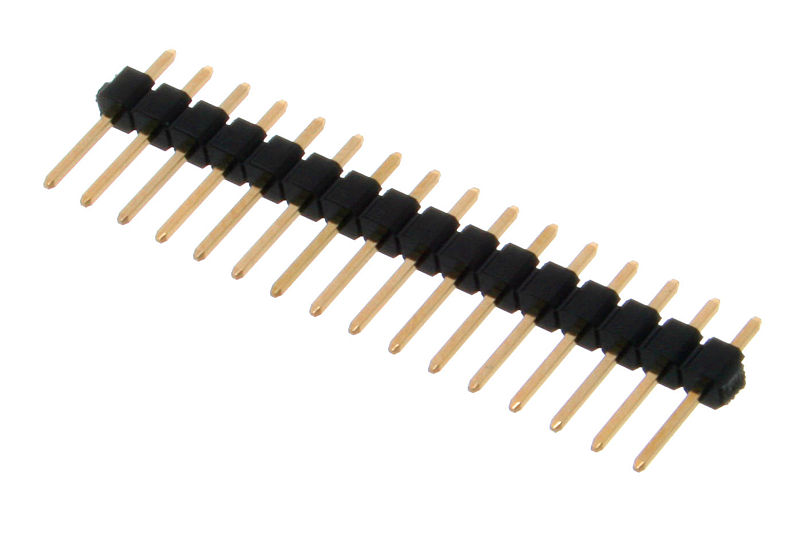
\includegraphics[width=0.07\textwidth]{tira_de_pines_simple.png}	

\end{itemize}

\subsubsection {Capacitores SMD-0805}
\begin{itemize}
\item $100nF$ (x7 Unidades)
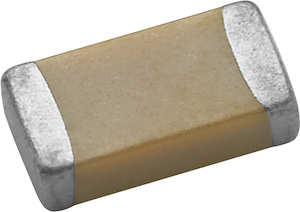
\includegraphics[width=0.03\textwidth]{capacitor_smd.png}	
\item $330nF$ (x1 Unidad)
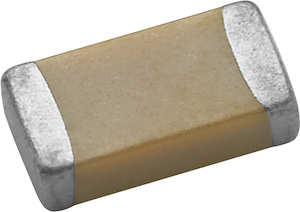
\includegraphics[width=0.03\textwidth]{capacitor_smd.png}	
\item $220\mu F$ (x1 Unidad, Polarizado Electrolítico)
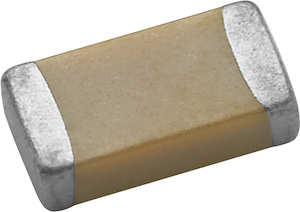
\includegraphics[width=0.03\textwidth]{capacitor_smd.png}	
\item $10\mu F$(x2 Unidades, Polarizado Electrolítico)
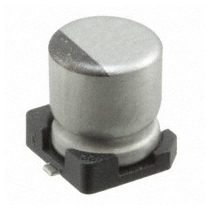
\includegraphics[width=0.03\textwidth]{capacitor_polarizado_smd.png}	
\item $1 \mu F$(x 1 Unidad, Polarizado Electrolítico)
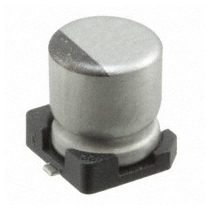
\includegraphics[width=0.03\textwidth]{capacitor_polarizado_smd.png}	
\end{itemize}
\subsubsection {Resistencias SMD-0805}
\begin{itemize}
\item $150\Omega$ (x3 Unidades)
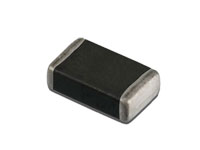
\includegraphics[width=0.03\textwidth]{resistencia_smd.png}	
\item $4,7K\Omega$(x1 Unidad)
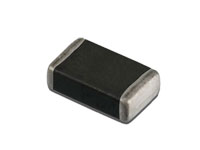
\includegraphics[width=0.03\textwidth]{resistencia_smd.png}	
\item $47K\Omega$(x1 Unidad)
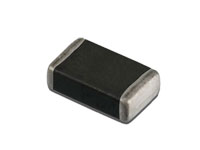
\includegraphics[width=0.03\textwidth]{resistencia_smd.png}	
\item $1K\Omega$(x2 Unidad)
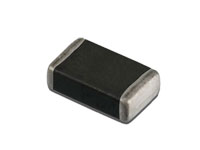
\includegraphics[width=0.03\textwidth]{resistencia_smd.png}	
\end{itemize}
\end{itemize}

\pagebreak

\section {Fuente de Alimentación}

\textsc{\Large Potencia disipada en $14,5V$:}

\begin{itemize}
\item Cooler's: $5,8 W$
\item HTC : $0,9 W$
\item Celda Peltier $69 W$
\end{itemize}
Total de potencia disipada en $14,5V$ $75,7W$

\textsc{\Large Potencia disipada en 12 V:}

\begin{itemize}
\item Motores DC $14,4 W$
\end{itemize}

Total de potencia disipada en $12V$ $12W$

Se requeriria una fuente que entregue minimamente $80W$ para la tension de $14,5V$ y $14W$ para la tension de $12V$.

\pagebreak

\section{Temperatura mínima}

Se busco la mínima temperatura que alcanza el gabinete dejando prendido el sistema de enfriamiento de tecnología Peltier por 19 horas y midiendo externamente su temperatura con una resolución de una muestra cada dos minutos. Dichos valores se graficaron obteniendo lo siguiente.

\begin{figure}[H]\label{temperatura_minima}
\centering
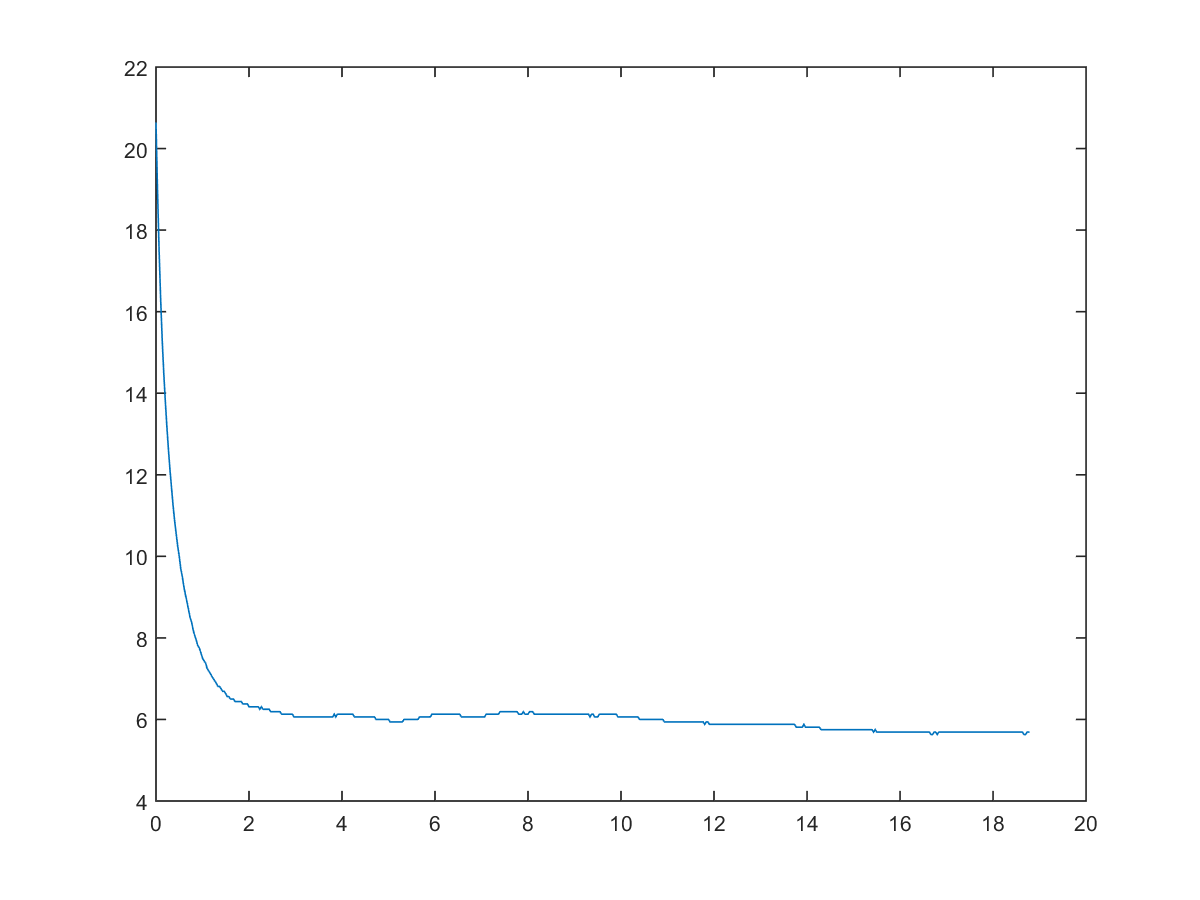
\includegraphics[width=0.8\textwidth]{temp_minima.png}
\caption{Grafico de la temperatura en función de las horas transcurridas.}
\end{figure}

El minimo alcazado es $5,65^{\circ} C$, siendo este su valor promedio asintotico, en 3 horas de funcionamiento dando una disminución de la temperatura a razón de $-5,58\frac{^{\circ}C}{Hora}$.

\pagebreak

\section{Temperatura de histéresis}

En este caso se fijo una temperatura de $10^{\circ} C$  con una toleracia $\pm 2^{\circ} C$, se tomaron valores externamente al igual que en el caso anterior y se obtuvo el siguiente gráfico.


\begin{figure}[H]\label{histeresis}
\centering
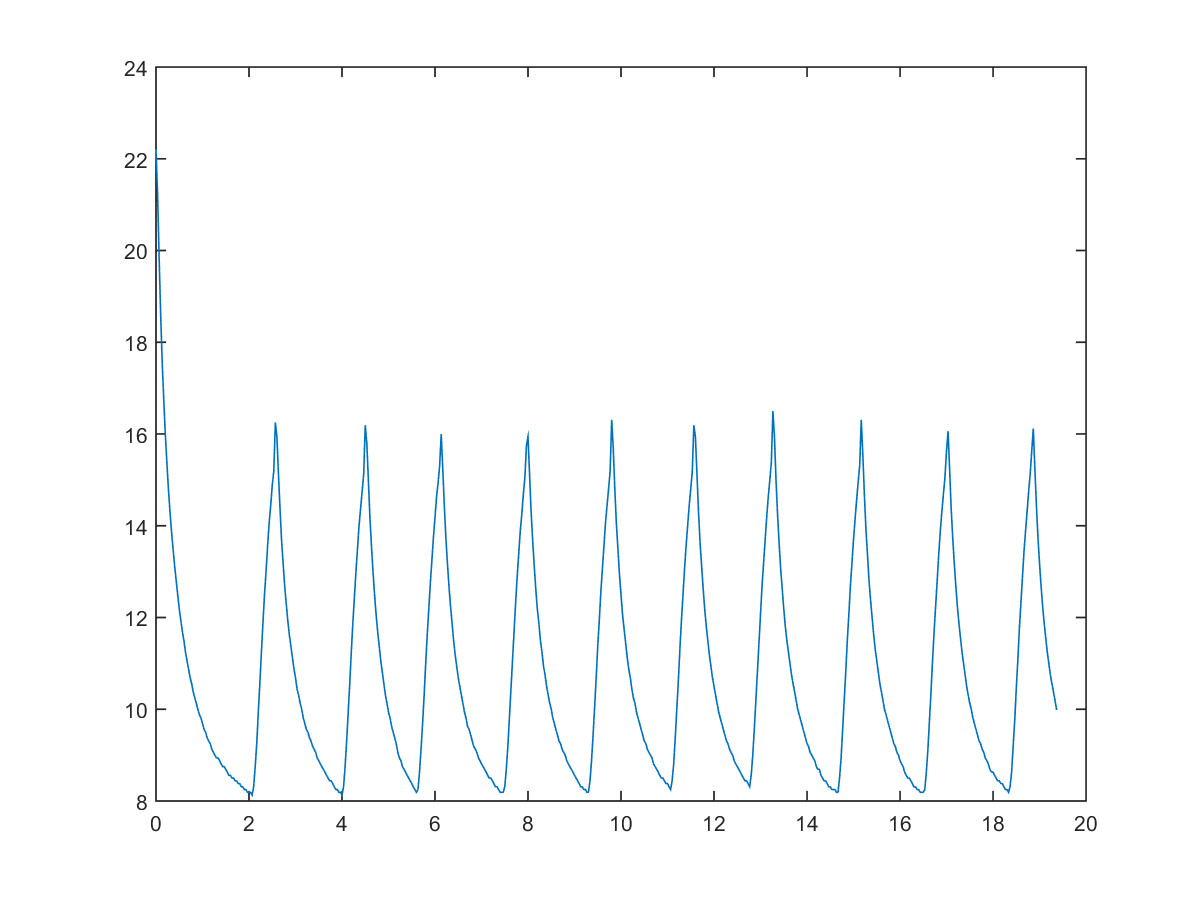
\includegraphics[width=0.8\textwidth]{histeresis.png}
\caption{Grafico de la temperatura en función de las horas transcurridas.}
\end{figure}

La temperatura promedio en la zona de oscilación es de $10,7^{\circ} C$.


\end{document}